\documentclass[aspectratio=169]{beamer}
\usepackage{color,amsmath}
\usepackage{subfigure}
\usepackage{booktabs}
\usepackage{framed}
\usepackage{comment}

\def\vf{\vfill}

%%%%%%%%%%%%%%%%%%%%%%%%%%
\title[]{Counting things (02-04)}
\author[]{Matthew J. Salganik\\Department of Sociology\\Princeton University}
\date[]{Soc 596: Computational Social Science
\vfill
\begin{flushright}
\vspace{0.6in}

\includegraphics[width=0.1\textwidth]{figures/cc.png}
\end{flushright}
}
\begin{document}
%%%%%%%%%%%%%%%%%%%%%%%%%%
\frame{\titlepage}
%%%%%%%%%%%%%%%%%%%%%%%%%%
\begin{frame}

Beneath the jargon and technical details, lots of research is just counting things.\\
\vf
\pause
What to count?
\begin{itemize}
\item Interesting
\item Important
\end{itemize}

\end{frame}
%%%%%%%%%%%%%%%%%%%%%%%%%%
\begin{frame}

\begin{itemize}
\item Theory-driven data analysis
\item Data-driven theorizing
\end{itemize}

\end{frame}
%%%%%%%%%%%%%%%%%%%%%%%%%%
\begin{frame}

\begin{center}
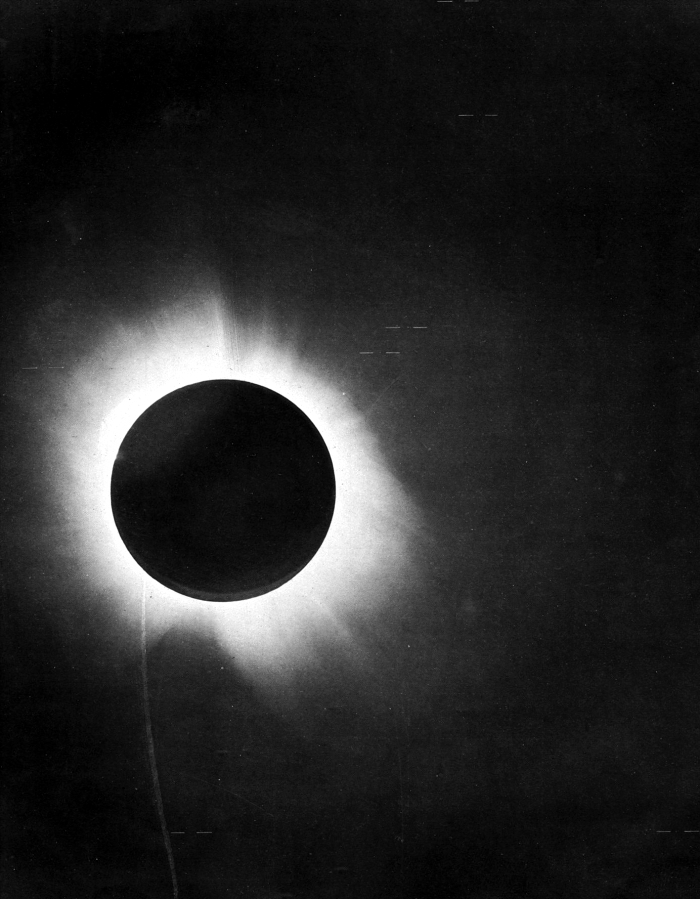
\includegraphics[height=0.6\textheight]{figures/1919_eclipse_positive}
\end{center}

What makes this interesting and important is not in the data itself
\vf
\TINY{\url{https://commons.wikimedia.org/wiki/File:1919_eclipse_positive.jpg}}

\end{frame}
%%%%%%%%%%%%%%%%%%%%%%%%%%
\begin{frame}

\begin{center}
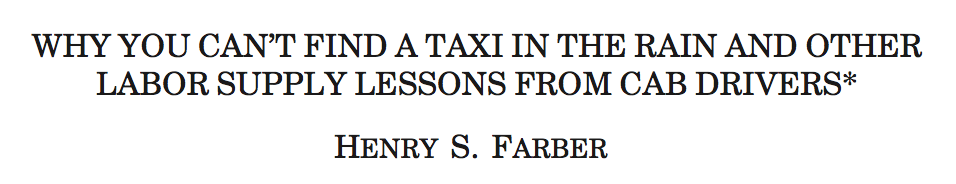
\includegraphics[width=\textwidth]{figures/farber_why_2015_title}
\end{center}

\vf
Farber 2015. ``Why you can't find a taxi in the rain and other labor supply lessons from cab drivers.'' \textit{Quarterly Journal of Economics}, \url{http://dx.doi.org/10.1093/qje/qjv026}

\end{frame}
%%%%%%%%%%%%%%%%%%%%%%%%%%
\begin{frame}

\begin{itemize}
\item Strategic research site (Merton)
\pause
\item Tests competing theory
\pause
\item replication and extension
\pause
\item Best-case for big data
\end{itemize}

\end{frame}
%%%%%%%%%%%%%%%%%%%%%%%%%%
\begin{frame}

Careful counting of hours worked and hourly wages\\
Better data leads to better estimate

\end{frame}
%%%%%%%%%%%%%%%%%%%%%%%%%%
\begin{frame}

{\Large
\begin{center}
How does he use the size of his data?
\end{center}
}
\pause
heterogeneity, mechanisms

\end{frame}
%%%%%%%%%%%%%%%%%%%%%%%%%%
\begin{frame}

{\Large
\begin{center}
Key ideas from social science:\\
heterogeneity, mechanisms
\end{center}
}

\end{frame}
%%%%%%%%%%%%%%%%%%%%%%%%%%
\begin{frame}

\begin{center}
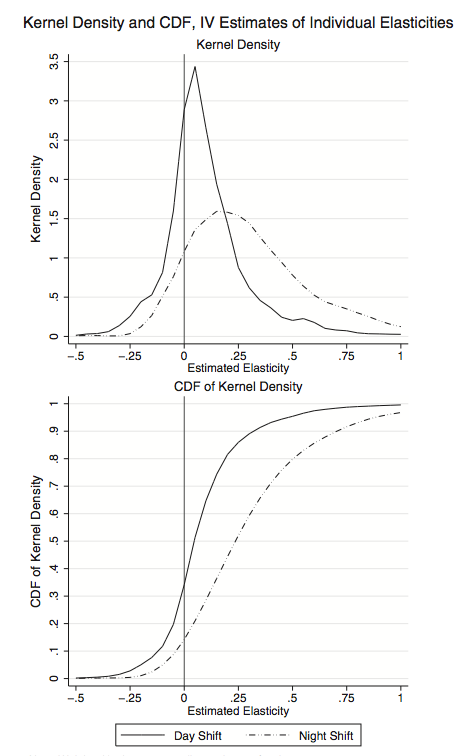
\includegraphics[height=0.8\textheight]{figures/farber_why_2015_fig6.png}
\end{center}

\end{frame}
%%%%%%%%%%%%%%%%%%%%%%%%%
\begin{frame}

\begin{center}
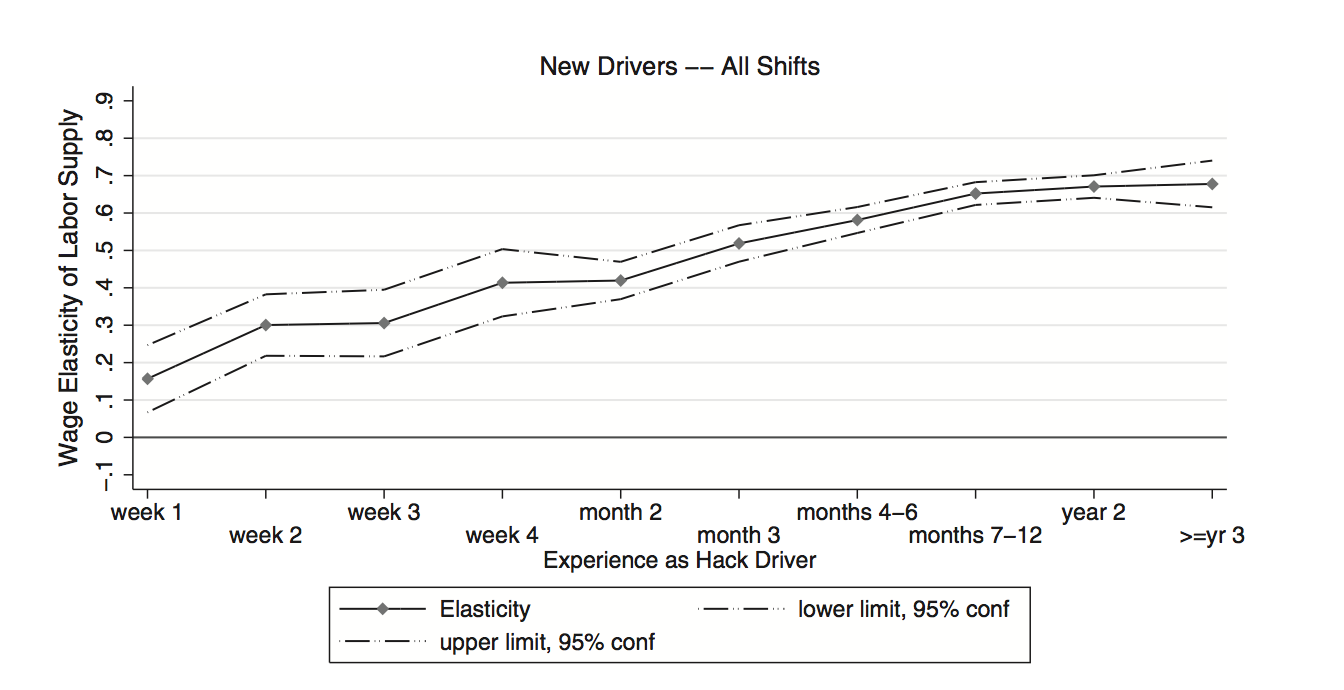
\includegraphics[width=\textwidth]{figures/farber_why_2015_fig7.png}
\end{center}

\end{frame}
%%%%%%%%%%%%%%%%%%%%%%%%%
\begin{frame}

Compare this to everything else people have done with NYC taxi data

\end{frame}
%%%%%%%%%%%%%%%%%%%%%%%%%%


\end{document}
